% Options for packages loaded elsewhere
\PassOptionsToPackage{unicode}{hyperref}
\PassOptionsToPackage{hyphens}{url}
%
\documentclass[
]{article}
\usepackage{amsmath,amssymb}
\usepackage{iftex}
\ifPDFTeX
  \usepackage[T1]{fontenc}
  \usepackage[utf8]{inputenc}
  \usepackage{textcomp} % provide euro and other symbols
\else % if luatex or xetex
  \usepackage{unicode-math} % this also loads fontspec
  \defaultfontfeatures{Scale=MatchLowercase}
  \defaultfontfeatures[\rmfamily]{Ligatures=TeX,Scale=1}
\fi
\usepackage{lmodern}
\ifPDFTeX\else
  % xetex/luatex font selection
\fi
% Use upquote if available, for straight quotes in verbatim environments
\IfFileExists{upquote.sty}{\usepackage{upquote}}{}
\IfFileExists{microtype.sty}{% use microtype if available
  \usepackage[]{microtype}
  \UseMicrotypeSet[protrusion]{basicmath} % disable protrusion for tt fonts
}{}
\makeatletter
\@ifundefined{KOMAClassName}{% if non-KOMA class
  \IfFileExists{parskip.sty}{%
    \usepackage{parskip}
  }{% else
    \setlength{\parindent}{0pt}
    \setlength{\parskip}{6pt plus 2pt minus 1pt}}
}{% if KOMA class
  \KOMAoptions{parskip=half}}
\makeatother
\usepackage{xcolor}
\usepackage[margin=1in]{geometry}
\usepackage{color}
\usepackage{fancyvrb}
\newcommand{\VerbBar}{|}
\newcommand{\VERB}{\Verb[commandchars=\\\{\}]}
\DefineVerbatimEnvironment{Highlighting}{Verbatim}{commandchars=\\\{\}}
% Add ',fontsize=\small' for more characters per line
\usepackage{framed}
\definecolor{shadecolor}{RGB}{248,248,248}
\newenvironment{Shaded}{\begin{snugshade}}{\end{snugshade}}
\newcommand{\AlertTok}[1]{\textcolor[rgb]{0.94,0.16,0.16}{#1}}
\newcommand{\AnnotationTok}[1]{\textcolor[rgb]{0.56,0.35,0.01}{\textbf{\textit{#1}}}}
\newcommand{\AttributeTok}[1]{\textcolor[rgb]{0.13,0.29,0.53}{#1}}
\newcommand{\BaseNTok}[1]{\textcolor[rgb]{0.00,0.00,0.81}{#1}}
\newcommand{\BuiltInTok}[1]{#1}
\newcommand{\CharTok}[1]{\textcolor[rgb]{0.31,0.60,0.02}{#1}}
\newcommand{\CommentTok}[1]{\textcolor[rgb]{0.56,0.35,0.01}{\textit{#1}}}
\newcommand{\CommentVarTok}[1]{\textcolor[rgb]{0.56,0.35,0.01}{\textbf{\textit{#1}}}}
\newcommand{\ConstantTok}[1]{\textcolor[rgb]{0.56,0.35,0.01}{#1}}
\newcommand{\ControlFlowTok}[1]{\textcolor[rgb]{0.13,0.29,0.53}{\textbf{#1}}}
\newcommand{\DataTypeTok}[1]{\textcolor[rgb]{0.13,0.29,0.53}{#1}}
\newcommand{\DecValTok}[1]{\textcolor[rgb]{0.00,0.00,0.81}{#1}}
\newcommand{\DocumentationTok}[1]{\textcolor[rgb]{0.56,0.35,0.01}{\textbf{\textit{#1}}}}
\newcommand{\ErrorTok}[1]{\textcolor[rgb]{0.64,0.00,0.00}{\textbf{#1}}}
\newcommand{\ExtensionTok}[1]{#1}
\newcommand{\FloatTok}[1]{\textcolor[rgb]{0.00,0.00,0.81}{#1}}
\newcommand{\FunctionTok}[1]{\textcolor[rgb]{0.13,0.29,0.53}{\textbf{#1}}}
\newcommand{\ImportTok}[1]{#1}
\newcommand{\InformationTok}[1]{\textcolor[rgb]{0.56,0.35,0.01}{\textbf{\textit{#1}}}}
\newcommand{\KeywordTok}[1]{\textcolor[rgb]{0.13,0.29,0.53}{\textbf{#1}}}
\newcommand{\NormalTok}[1]{#1}
\newcommand{\OperatorTok}[1]{\textcolor[rgb]{0.81,0.36,0.00}{\textbf{#1}}}
\newcommand{\OtherTok}[1]{\textcolor[rgb]{0.56,0.35,0.01}{#1}}
\newcommand{\PreprocessorTok}[1]{\textcolor[rgb]{0.56,0.35,0.01}{\textit{#1}}}
\newcommand{\RegionMarkerTok}[1]{#1}
\newcommand{\SpecialCharTok}[1]{\textcolor[rgb]{0.81,0.36,0.00}{\textbf{#1}}}
\newcommand{\SpecialStringTok}[1]{\textcolor[rgb]{0.31,0.60,0.02}{#1}}
\newcommand{\StringTok}[1]{\textcolor[rgb]{0.31,0.60,0.02}{#1}}
\newcommand{\VariableTok}[1]{\textcolor[rgb]{0.00,0.00,0.00}{#1}}
\newcommand{\VerbatimStringTok}[1]{\textcolor[rgb]{0.31,0.60,0.02}{#1}}
\newcommand{\WarningTok}[1]{\textcolor[rgb]{0.56,0.35,0.01}{\textbf{\textit{#1}}}}
\usepackage{graphicx}
\makeatletter
\def\maxwidth{\ifdim\Gin@nat@width>\linewidth\linewidth\else\Gin@nat@width\fi}
\def\maxheight{\ifdim\Gin@nat@height>\textheight\textheight\else\Gin@nat@height\fi}
\makeatother
% Scale images if necessary, so that they will not overflow the page
% margins by default, and it is still possible to overwrite the defaults
% using explicit options in \includegraphics[width, height, ...]{}
\setkeys{Gin}{width=\maxwidth,height=\maxheight,keepaspectratio}
% Set default figure placement to htbp
\makeatletter
\def\fps@figure{htbp}
\makeatother
\setlength{\emergencystretch}{3em} % prevent overfull lines
\providecommand{\tightlist}{%
  \setlength{\itemsep}{0pt}\setlength{\parskip}{0pt}}
\setcounter{secnumdepth}{-\maxdimen} % remove section numbering
\ifLuaTeX
  \usepackage{selnolig}  % disable illegal ligatures
\fi
\usepackage{bookmark}
\IfFileExists{xurl.sty}{\usepackage{xurl}}{} % add URL line breaks if available
\urlstyle{same}
\hypersetup{
  pdftitle={Cutoff Value Determination \& Graph},
  pdfauthor={Lea R. Medeiros},
  hidelinks,
  pdfcreator={LaTeX via pandoc}}

\title{Cutoff Value Determination \& Graph}
\author{Lea R. Medeiros}
\date{2025-03-18}

\begin{document}
\maketitle

\section{cutoffvalue}\label{cutoffvalue}

Cutoffvalue is a simple R package that implements an updated version of
the method first developed and used in Medeiros et al.~(2018). It can be
used to determine an objective cutoff value between a significantly
bimodal distribution of log-transformed data and plot a representative
graph of the results.

\subsection{Installation}\label{installation}

You can install the development version of cutoffvalue from
\href{https://github.com/lea-medeiros/cutoffvalue.git}{GitHub} with:

\begin{Shaded}
\begin{Highlighting}[]
\CommentTok{\# install.packages("devtools")}
\NormalTok{devtools}\SpecialCharTok{::}\FunctionTok{install\_github}\NormalTok{(}\StringTok{"lea{-}medeiros/cutoffvalue"}\NormalTok{)}
\end{Highlighting}
\end{Shaded}

\subsection{Example}\label{example}

This is a basic example which shows you how to use the cutoffvalue
package.

\subsubsection{Setup RStudio}\label{setup-rstudio}

Load the packages that are used by this package.

\begin{Shaded}
\begin{Highlighting}[]
\FunctionTok{library}\NormalTok{(cutoffvalue)}
\FunctionTok{library}\NormalTok{(mixtools)}
\FunctionTok{library}\NormalTok{(Hmisc)}
\FunctionTok{library}\NormalTok{(plyr)}
\FunctionTok{library}\NormalTok{(multimode)}
\FunctionTok{library}\NormalTok{(readxl)}
\end{Highlighting}
\end{Shaded}

\subsubsection{Define your raw dataset}\label{define-your-raw-dataset}

Specify the data file to be used in the analyses and graph (if located
in root folder of an R project, path information is not necessary).
Reminder: data should be organized in as a single column of log- or
natural log-transformed data without a column header.

\begin{Shaded}
\begin{Highlighting}[]
\NormalTok{mydata }\OtherTok{\textless{}{-}} \StringTok{"R/exampledata.xlsx"}
\end{Highlighting}
\end{Shaded}

\emph{This step isn't necessary if you'd rather use the path name for
your data.}

\subsubsection{Import the raw dataset}\label{import-the-raw-dataset}

Import data and remove rows containing NA data. This function also
defines minimum and maximum values for the dataset. The default for each
function is specified as ``R/exampledata.xlsx'', meaning that running
any function without specifying the dataset will use the
exampledata.xlsx file.

\begin{Shaded}
\begin{Highlighting}[]
\NormalTok{mydata }\OtherTok{\textless{}{-}} \FunctionTok{importdata}\NormalTok{()}
\end{Highlighting}
\end{Shaded}

\emph{Alternatively, you could enter the path name of your data in the
read\_excel function}

\subsubsection{Determine modality}\label{determine-modality}

Determine if the data is not unimodal (e.g., bimodal). This function
also returns the Excess Mass statistic and associated p-value in the
Environment.

\begin{Shaded}
\begin{Highlighting}[]
\NormalTok{modetest }\OtherTok{\textless{}{-}} \FunctionTok{modes}\NormalTok{()}
\end{Highlighting}
\end{Shaded}

\begin{verbatim}
## Modality Test Results
## 
## P-value: 0.002 
## Excess Mass Statistic: 0.09846337 
## **Reject null hypothesis** Distribution contains more than one mode; proceed with analyses.
## 
## Test Credit: Ameijeiras-Alonso et al. (2019) excess mass test
\end{verbatim}

\emph{Returns excess mass statistic and p-value. If the p-value is less
than 0.05, accept the alternative hypothesis (data is more than
unimodal) and proceed with analysis. However, if the p-value is more
than 0.05, the data is unimodal and the following analyses are not
entirely valid.}

\subsubsection{Fit a model to the data}\label{fit-a-model-to-the-data}

Fit the two component mixture models to the data and plot a rough
histogram with the fitted lines. Also, define the index.lower value to
be used in the find.cutoff function.

\begin{Shaded}
\begin{Highlighting}[]
\NormalTok{Mcmodel }\OtherTok{\textless{}{-}} \FunctionTok{datamodel}\NormalTok{()}
\end{Highlighting}
\end{Shaded}

\begin{center}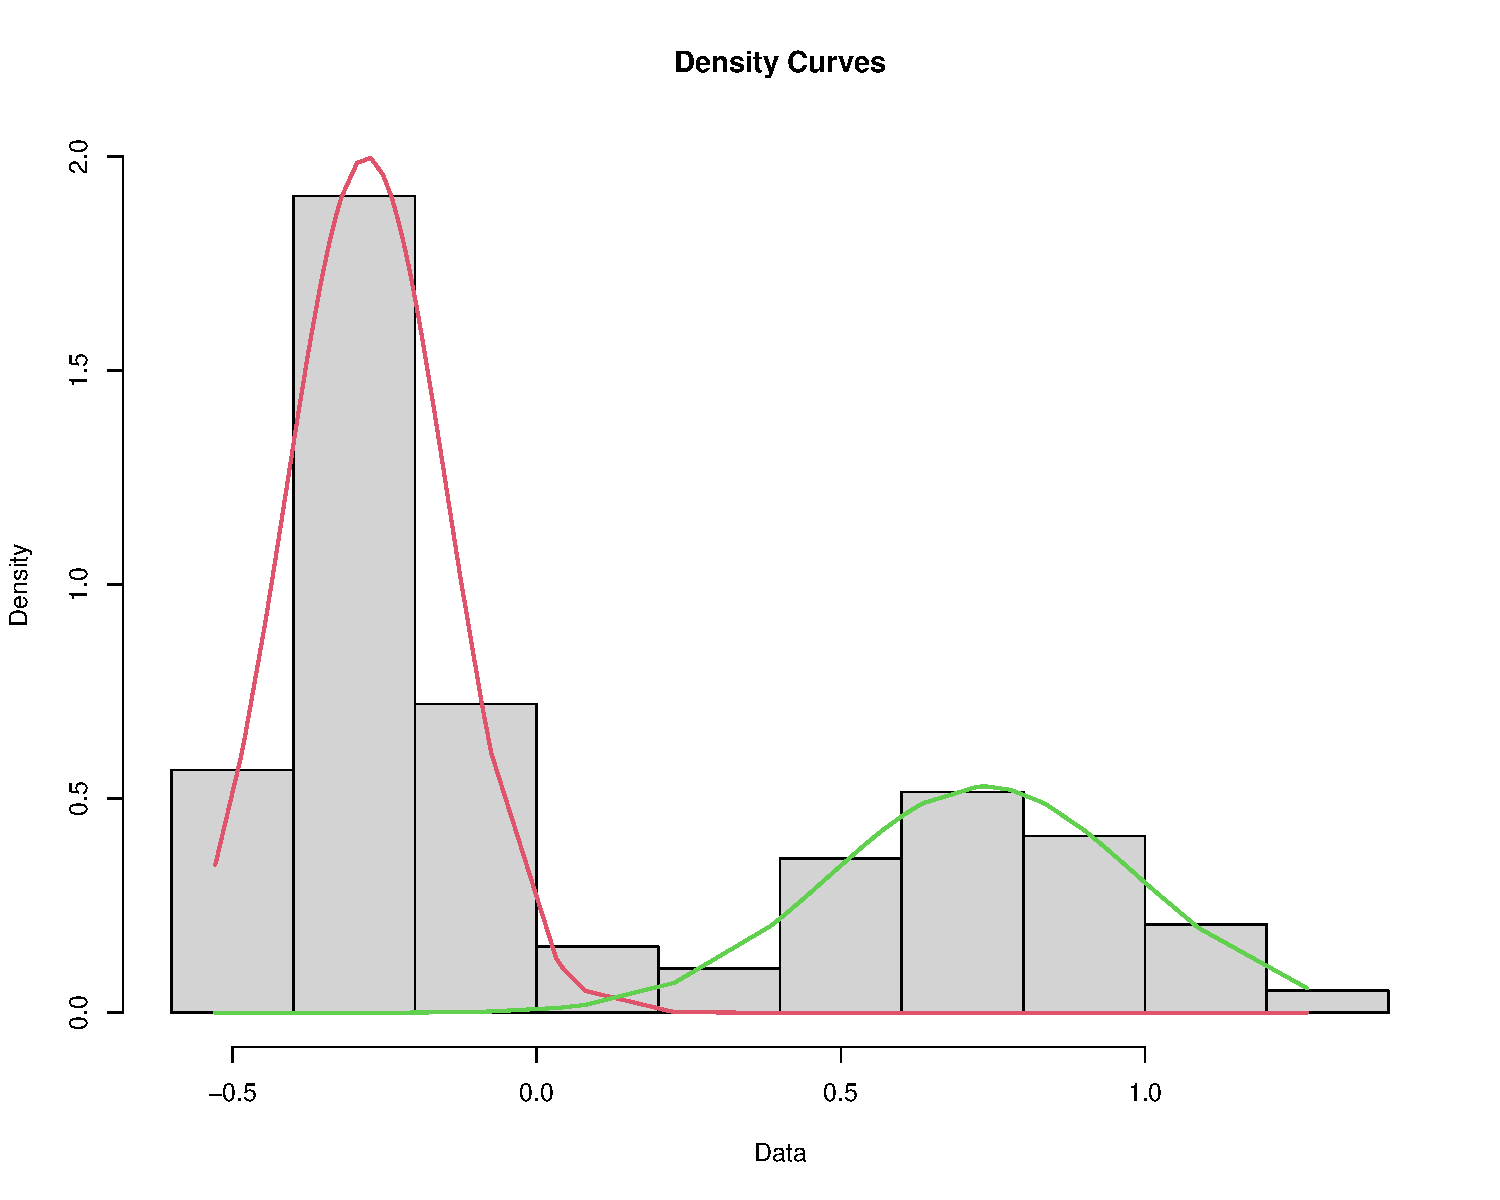
\includegraphics{man/cutoffvalue_figures/README-model-data-1} \end{center}

\emph{Make sure things look right, but won't actually use this graph as
it plots on a density scale and may cause confusion. However, this
should look pretty spot on (final graph will just be scaled up by a
constant determined later on), so make sure that the point where the two
curves intersect is where you are expecting the cutoff to be.}

\subsubsection{Determine the cutoff
value}\label{determine-the-cutoff-value}

Determine the cutoff value between the two populations that has an equal
chance of being drawn from either mode. The default is 0.5, but the
probability can be changed in the code.

\begin{Shaded}
\begin{Highlighting}[]
\NormalTok{cutoff }\OtherTok{\textless{}{-}} \FunctionTok{findcutoff}\NormalTok{()}
\end{Highlighting}
\end{Shaded}

\begin{verbatim}
## [1] 0.1124714
\end{verbatim}

\emph{The uniroot lower and upper values are determined using the range
of ``mydata'' and will reflect the dataset being analyzed. If there are
errors due to the uniroot, consider editing the custom values to
something that more generally reflects the range of the data being
analyzed.}

\subsubsection{Basic histogram and
parameters}\label{basic-histogram-and-parameters}

The code below will produce basic histogram of data used for the
parameters it produces; alter number of breaks to reflect what you would
like to see in the final graph. Then, use various parameters to define
variables for the final graph

\begin{Shaded}
\begin{Highlighting}[]
\NormalTok{fit }\OtherTok{\textless{}{-}} \FunctionTok{fitparams}\NormalTok{()}
\end{Highlighting}
\end{Shaded}

\begin{center}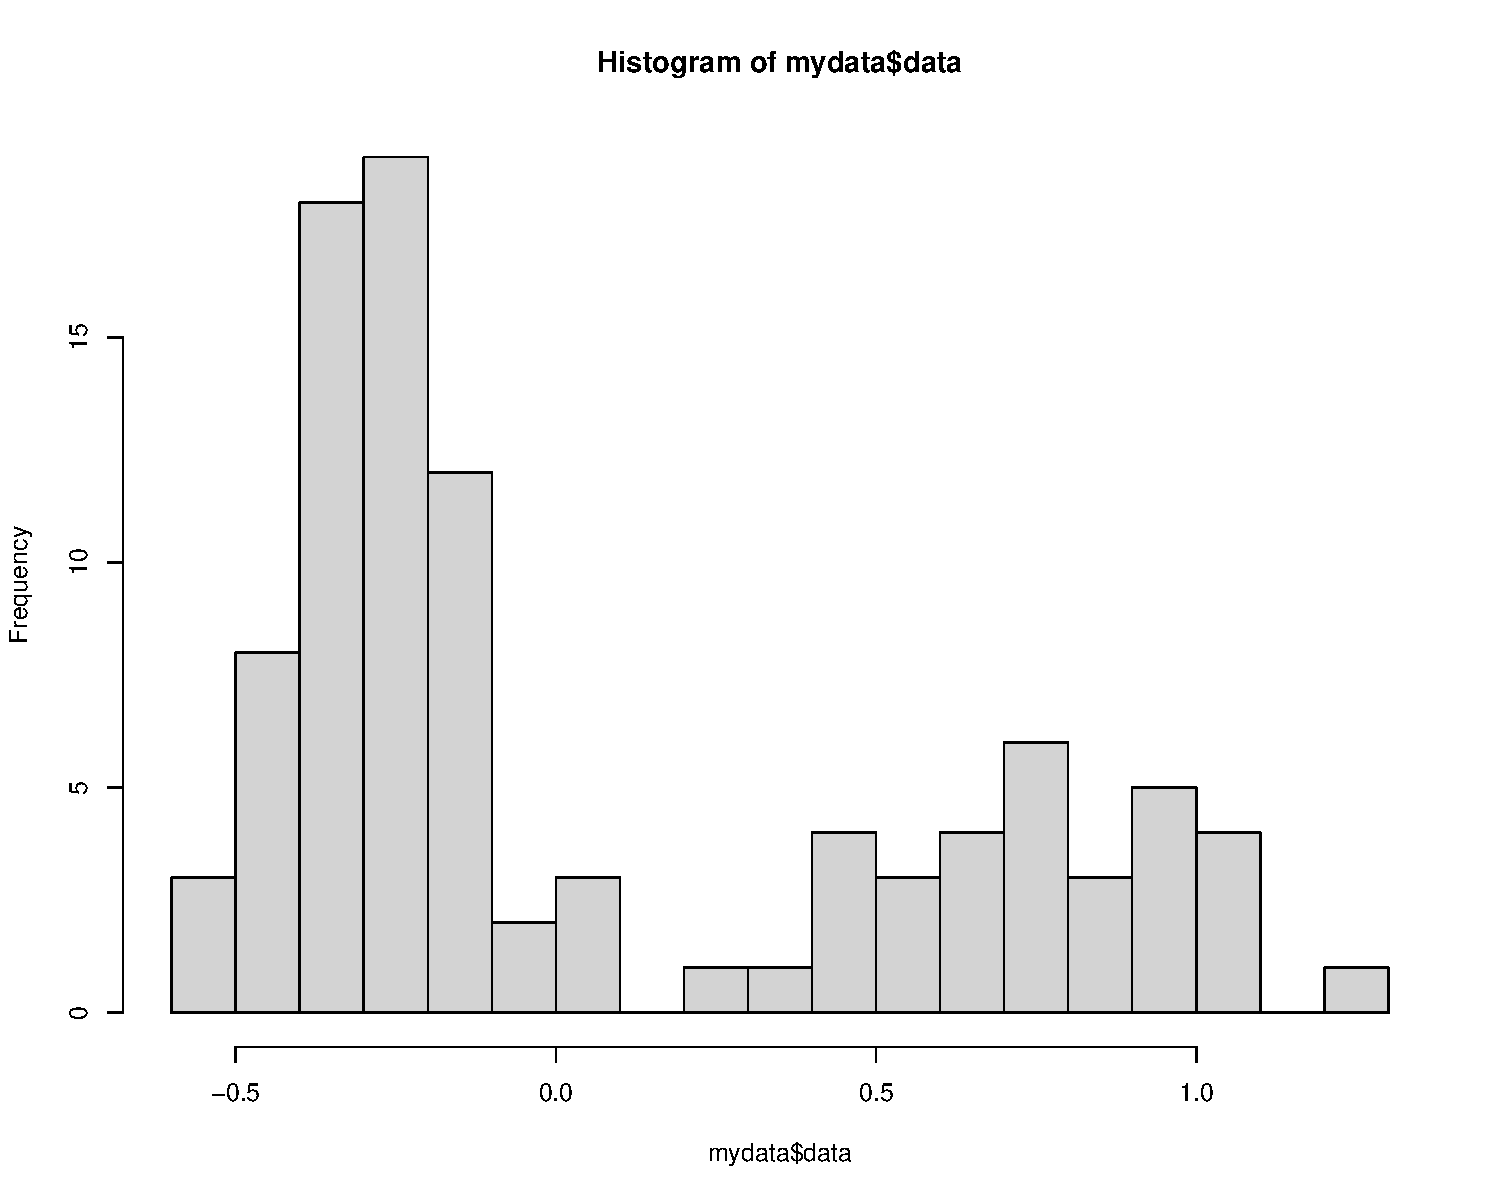
\includegraphics{man/cutoffvalue_figures/README-basic-histogram-1} \end{center}

\subsubsection{Create curves}\label{create-curves}

Determine x and y values to calculate the points for the curves to
represent the generated models

\begin{Shaded}
\begin{Highlighting}[]
\NormalTok{curves }\OtherTok{\textless{}{-}} \FunctionTok{curves}\NormalTok{()}
\end{Highlighting}
\end{Shaded}

\emph{Creates curves using model parameters}

\subsubsection{Plot the graph}\label{plot-the-graph}

Plot a pretty graph - SOME OF THE FOLLOWING WILL NEED TO BE TWEAKED TO
FIT YOUR DATA/PREFERENCES!!! If nothing is specified in the plot
function, then these are used.

\paragraph{Specify graph labels}\label{specify-graph-labels}

\begin{Shaded}
\begin{Highlighting}[]
\NormalTok{title }\OtherTok{\textless{}{-}} \StringTok{"Plasma 11{-}KT levels in age{-}2 male spring chinook"}  \CommentTok{\# Graph title}
\NormalTok{xlab }\OtherTok{\textless{}{-}} \StringTok{"Plasma [11{-}KT] (ng/mL)"} \CommentTok{\# X{-}axis label}
\NormalTok{cutofflab }\OtherTok{\textless{}{-}} \StringTok{"Minijack cutoff"} \CommentTok{\# label for cutoff value on graph}
\NormalTok{cutoffunits }\OtherTok{\textless{}{-}} \StringTok{"(ng/mL)"} \CommentTok{\# units for cutoff value}
\end{Highlighting}
\end{Shaded}

\paragraph{Plot the graph}\label{plot-the-graph-1}

\begin{Shaded}
\begin{Highlighting}[]
\NormalTok{plottyMcplotty }\OtherTok{\textless{}{-}} \FunctionTok{cutoffplot}\NormalTok{(mydata, title, xlab, cutofflab, cutoffunits)}
\end{Highlighting}
\end{Shaded}

\begin{center}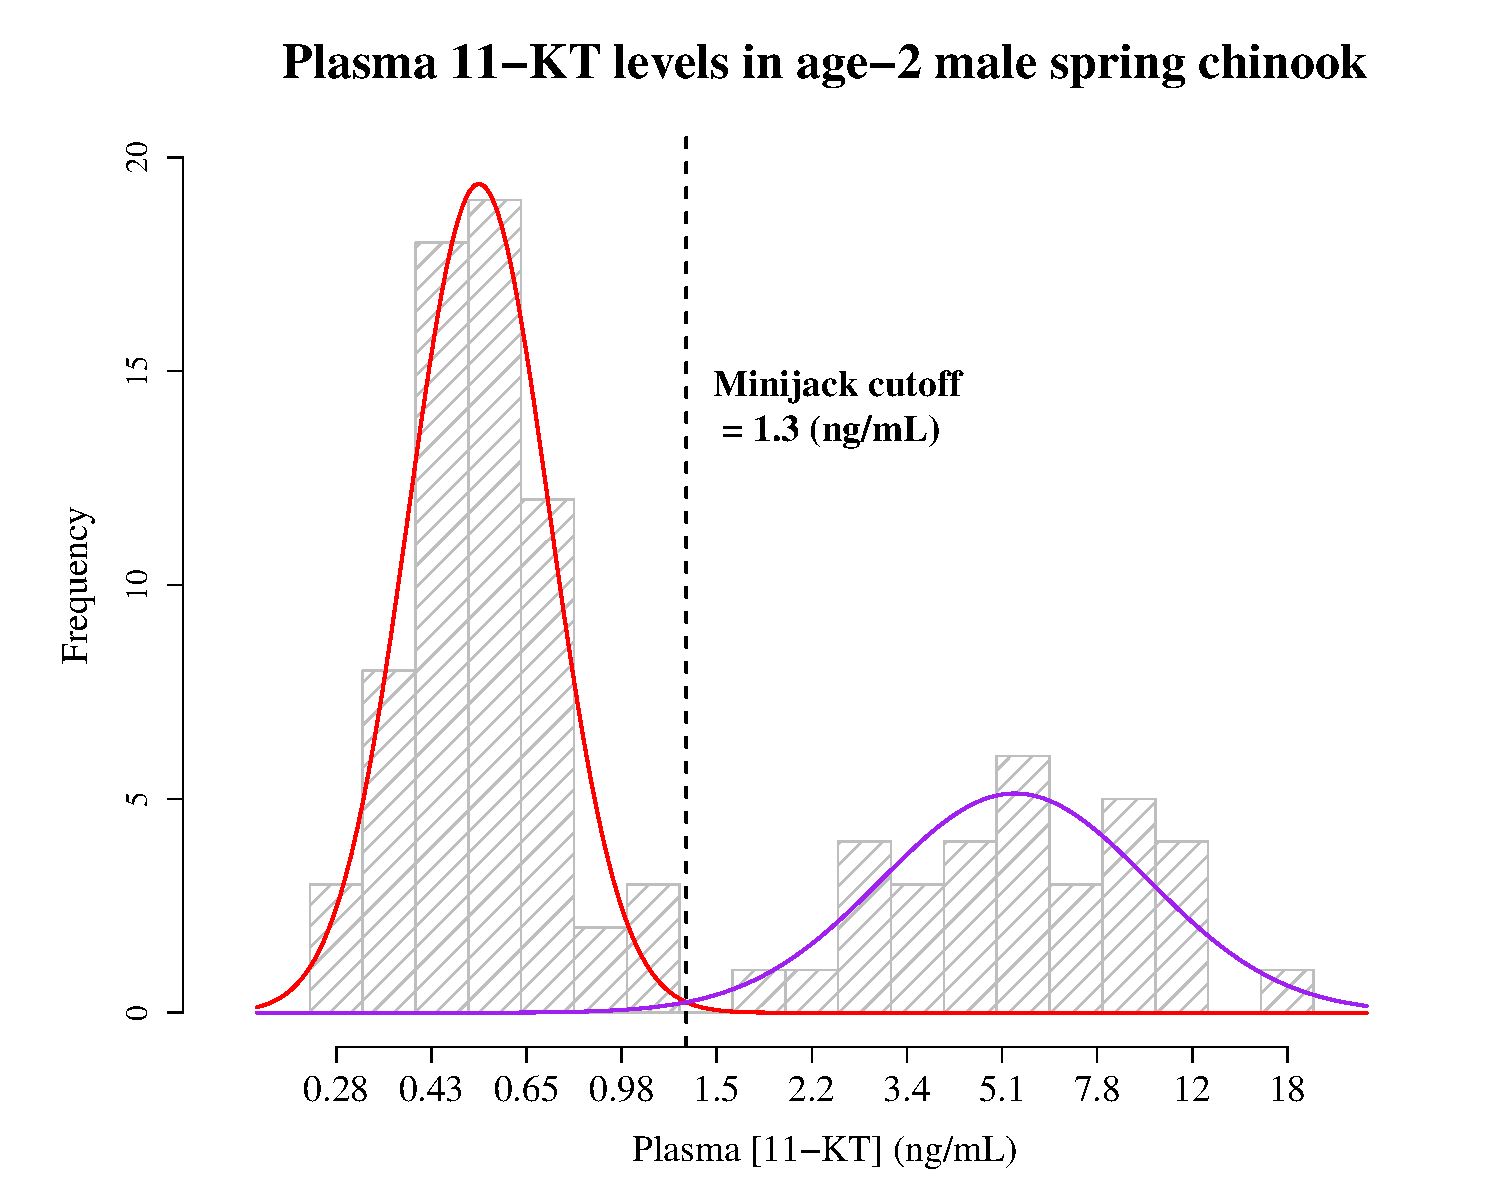
\includegraphics{man/cutoffvalue_figures/README-pretty_graph-1} \end{center}

\emph{All figures can be found in the ``cutoffvalue\_figures'' folder.
They are exported as PDF, JPEG, and PNG at 300 dpi.}

\end{document}
